\section{Neural Network Modeling}
\label{NN}

As it has been stated in the introduction, the modeling of the CHP plant described in the previous section has been performed by means of  NNs. In particular, we have adopted a divide-and-conquer strategy. That is, we have modeled each main component of the plant separately with an NN, and then, we have linked (connected) all the networks by means of shared or common variables (e.g.; an output variable of a network can be an input variable of one or several other networks). The global model is shown in Figure \ref{fignns} where a total of twelve NNs are depicted: four for the engines, four for the engine cooling  circuits, one for the exhaust steam boiler, one for the steam turbine condenser, one for the steam turbine and finally another one for the slurry drying process. All the NNs are actually multilayer perceptrons with just one hidden layer. In all of them, the number of neurons of the hidden layer is twice the number of inputs and there is only one neuron in the output layer (i.e., each NN computes just a single output value). These outputs are respectively: a) the temperature of the water to cool each engine ($T_{Mixt\_EngA}, \dots, T_{Mixt\_EngD}$; b) the flow of fuel (i.e. natural gas) required by each engine ($F_{Gas_A} \dots F_{Gas_D}$); c) the pressure of the condenser ($P_{CON}$); d) the steam flow in the boiler ($F_{Steam}$); e) the electric power produced by the turbine ($POW_{ST}$) and f) the flow of slurry processed by the evaporator ($F_{EV}$). 

To train and test the NNs, a big data set was collected trough a one-year observation process in the real plant. 213 parameters were identified as being potentially relevant for training and validating the NN models. Their values have been measured and retrieved with a resolution of one minute during the whole period of observation. Firstly, a careful analysis of the data was performed to choose the most relevant variables and also to filter outliers, missing data or un-informative variables. Next, based on previous knowledge of the system physics and also on a trial/error process, the particular variables for each model were fixed. Figure \ref{fignns} shows these input/output variables for the different NNs. The variables written in bold refer to the decision variables that are used in the optimization process. Finally, from the whole data set, we have chosen 10-minute separated values, because we observed that the variables change very little in a minute, due to the slow dynamics of the plant. Therefore we have a total of about \num{40000} samples, half of which were used to train the networks and the other half to test the modeling performance. To train the NNs the Back-Propagation algorithm was used, which, depending on the case, needed between \num{4000} and \num{20000} iterations to perform the learning process (i.e. until the error was stabilized and it was lower than a threshold). The whole modeling process has been carried out by using the Optibat trainer Tool (\cite{Optibat}).

\begin{figure}
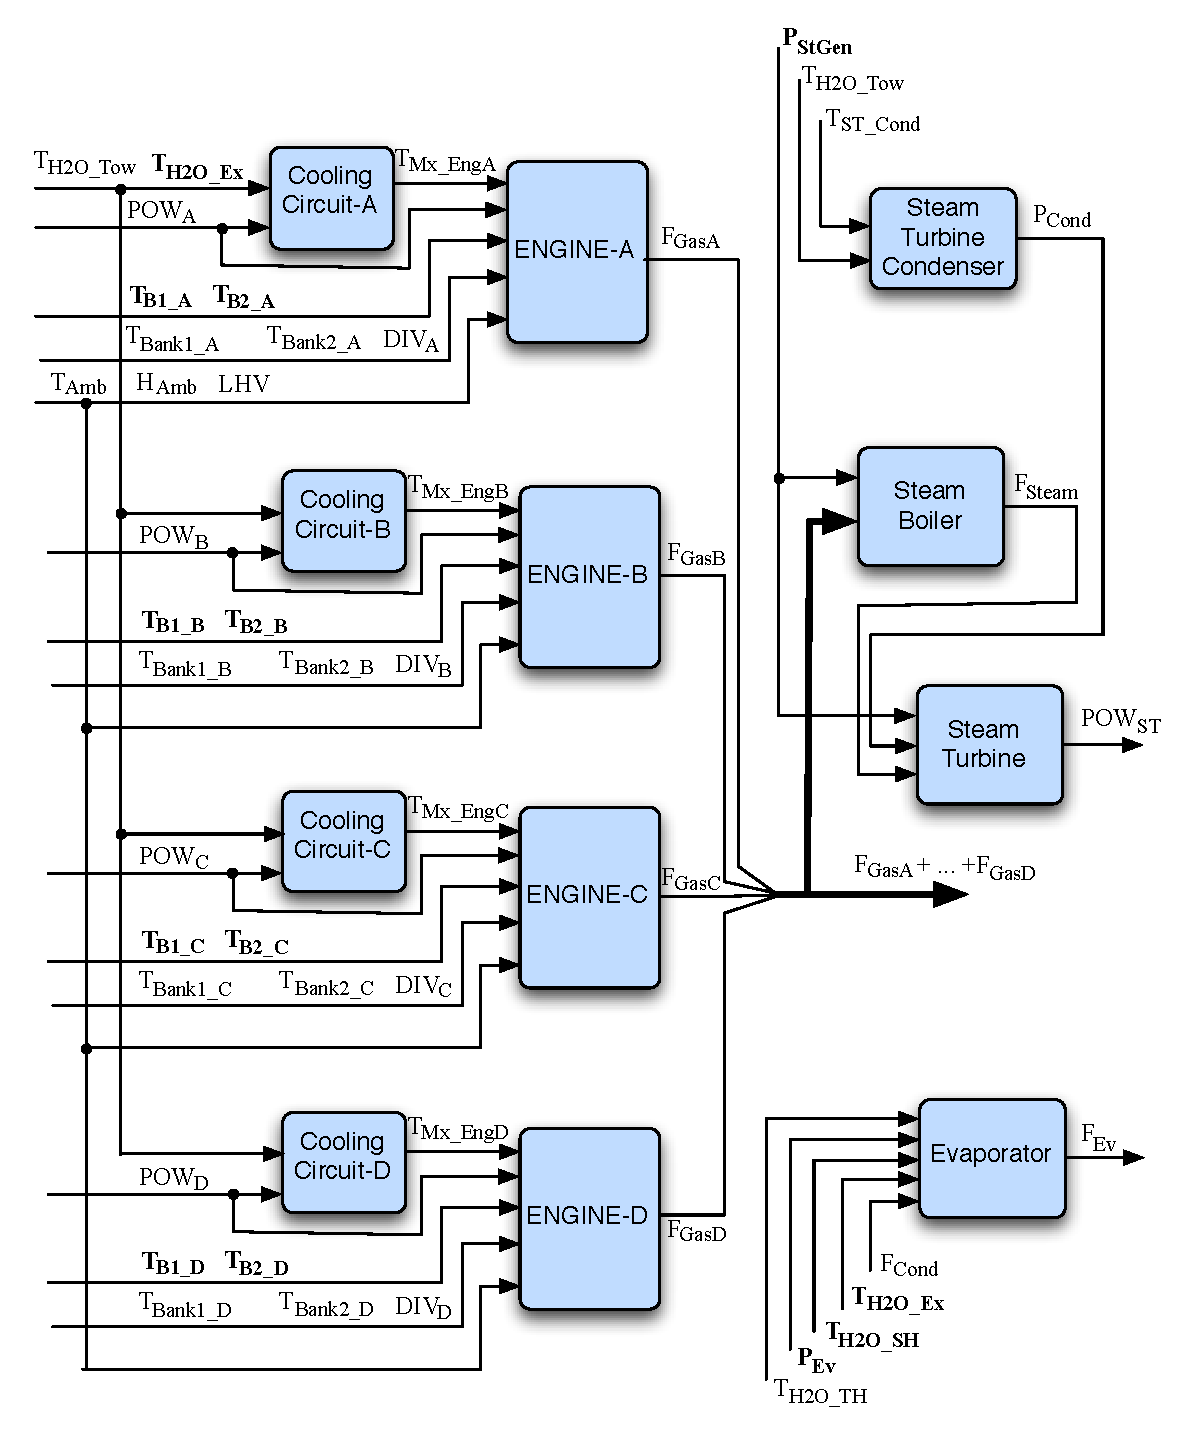
\includegraphics[width=1\textwidth]{NNs.pdf}
\caption{Modeling of the CHP Plant by means of interconnected NNs. Each block represents an NN.}
\label{fignns}
\end{figure}


The result of the modeling is presented in Table \ref{tbl:mse}, where the mean squared error (MSE) between the desired and actual output, for both the training and the testing phase, is shown. We can see that, in all the cases, the obtained  errors are very small, even in the testing case, where the NNs deal with unseen data. These results validate the modeling performance of the trained NNs. 

\begin{table}[!t]
\caption{MSE for training and testing samples for each Neural Network.}
\label{tbl:mse}
  \centering
\begin{tabular}{lrrrr} \toprule
 & Structure* & Iterations & Train Error & Test Error \\ \midrule
Cooling Engine A & 3/6/1 & \num{6000} & \SI{0.21}{\percent} & \SI{0.23}{\percent} \\
Cooling Engine B & 3/6/1 & \num{6000} & \SI{0.28}{\percent} & \SI{0.26}{\percent} \\
Cooling Engine C & 3/6/1 & \num{6000} & \SI{0.10}{\percent} & \SI{0.13}{\percent} \\
Cooling Engine D & 3/6/1 & \num{6000} & \SI{0.49}{\percent} & \SI{0.33}{\percent} \\
 Engine A & 10/20/1 & \num{20000} & \SI{0.39}{\percent} & \SI{0.42}{\percent} \\
 Engine B & 10/20/1 & \num{20000} & \SI{0.41}{\percent} & \SI{0.41}{\percent} \\
 Engine C & 10/20/1 & \num{20000} & \SI{0.38}{\percent} & \SI{0.42}{\percent} \\
 Engine D & 10/20/1 & \num{20000} & \SI{0.38}{\percent} & \SI{0.37}{\percent} \\
 Recovery Boiler & 2/4/1 & \num{4000} & \SI{0.61}{\percent} & \SI{0.63}{\percent} \\
 Steam Condenser & 2/4/1 & \num{4000} & \SI{1.01}{\percent} & \SI{0.96}{\percent} \\
 Steam Turbine & 3/6/1 & \num{6000} & \SI{0.67}{\percent} & \SI{0.70}{\percent} \\
 Slurry Process & 5/10/1 & \num{10000} & \SI{2.35}{\percent} & \SI{2.52}{\percent} \\
 \bottomrule
\end{tabular}
\vspace{-0.3cm}

\end{table}


For better appreciating the predicting ability of the NNs, we have also plotted the predicted data and the real data for the testing points. Because the four cooling-circuit models and the four engine models have  similar behavior, we have plotted only the output variables of six of the twelve models: $T_{Mixt\_EngA}$, $F_{GasD}$, $P_{Cond}$, $F_{Steam}$, $POW_{ST}$ and $F_{Ev}$. Furthermore, due to the large amount of samples, the points are re-sampled every 30 minutes for the graphics. We can observe how the  real and predicted curves are quite similar in all the examples, confirming thus that the NNs are able to learn properly the dynamics of the plant.


\begin{figure}
\centering
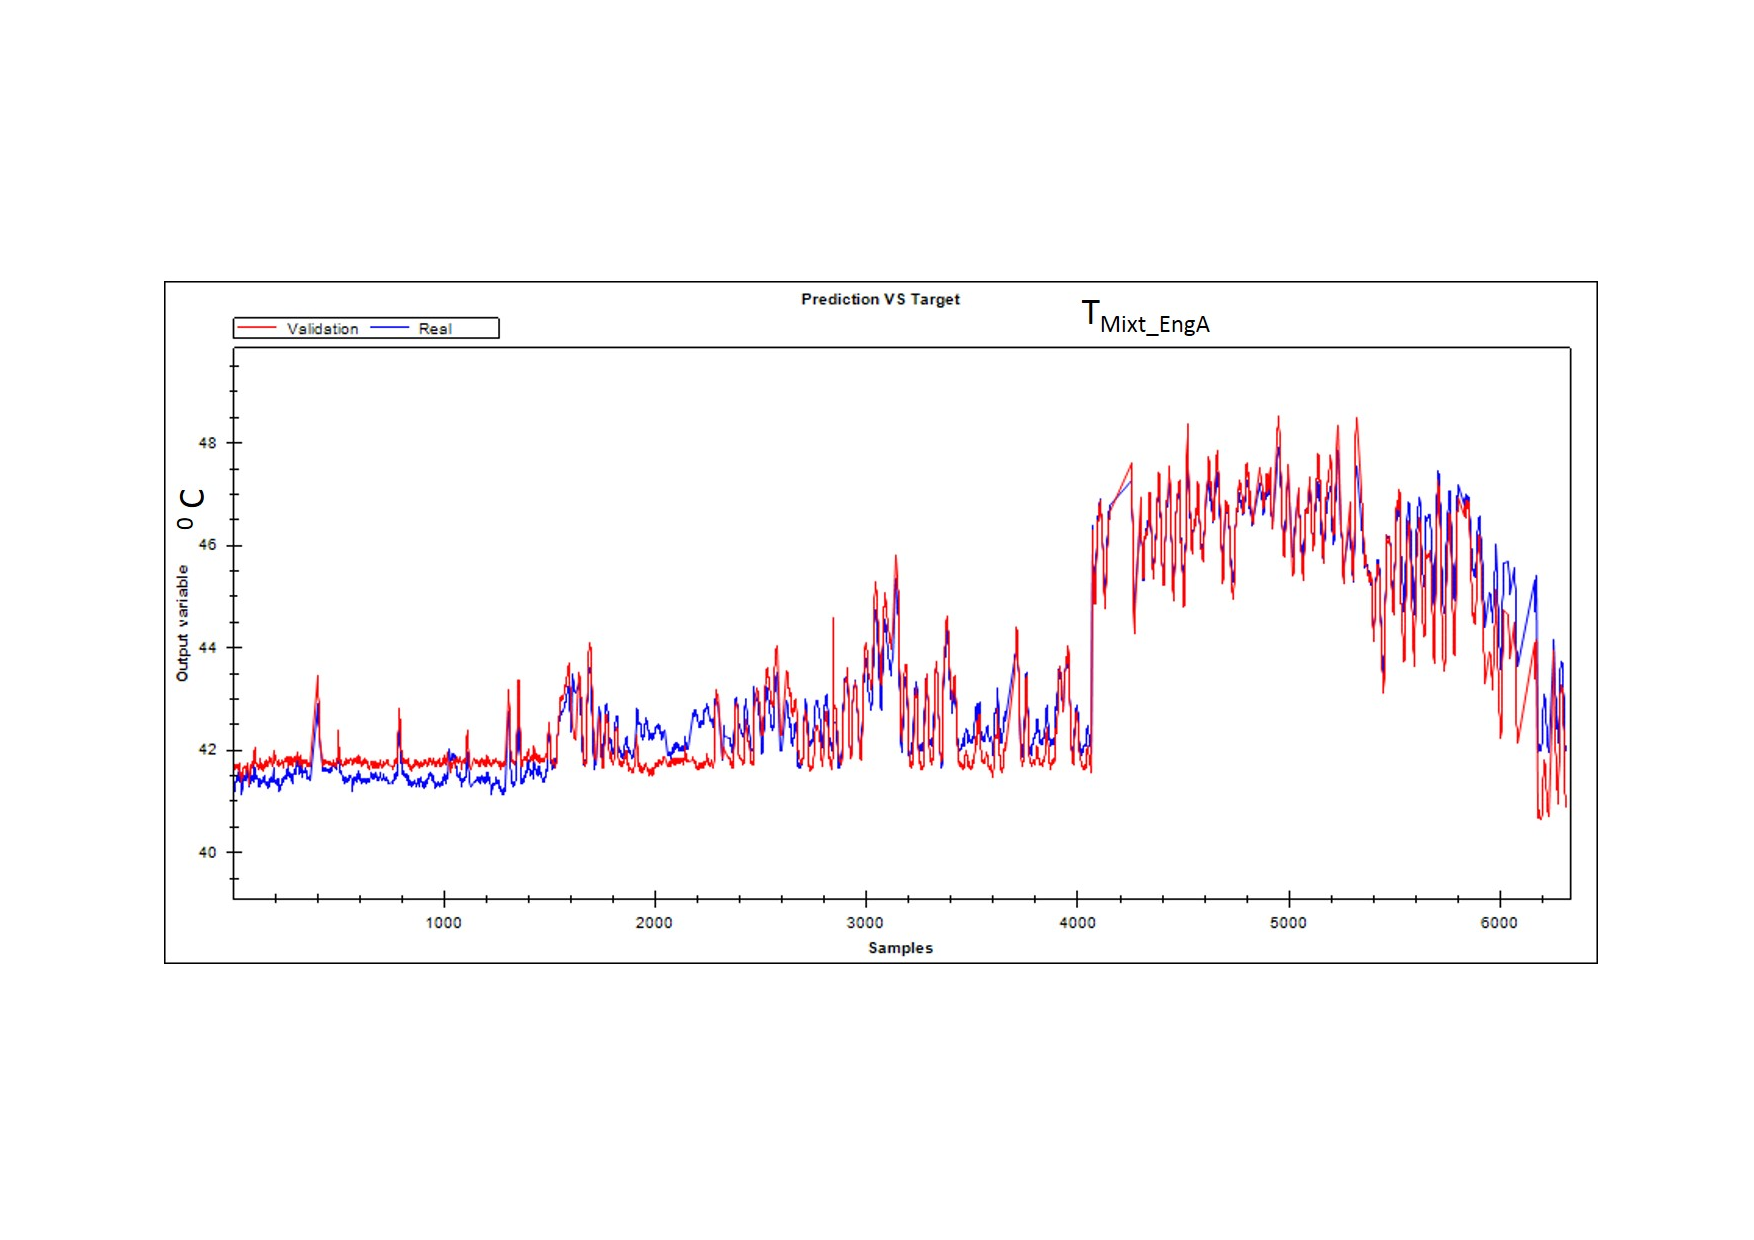
\includegraphics[width=1\textwidth]{IrrigationA-ANN.pdf}
\caption{Real data and NN predicted data for the cooling circuit temperature of Engine A ($T_{Mixt\_EngA}$).}
\label{TcoolA}
\end{figure}

\begin{figure}
\centering
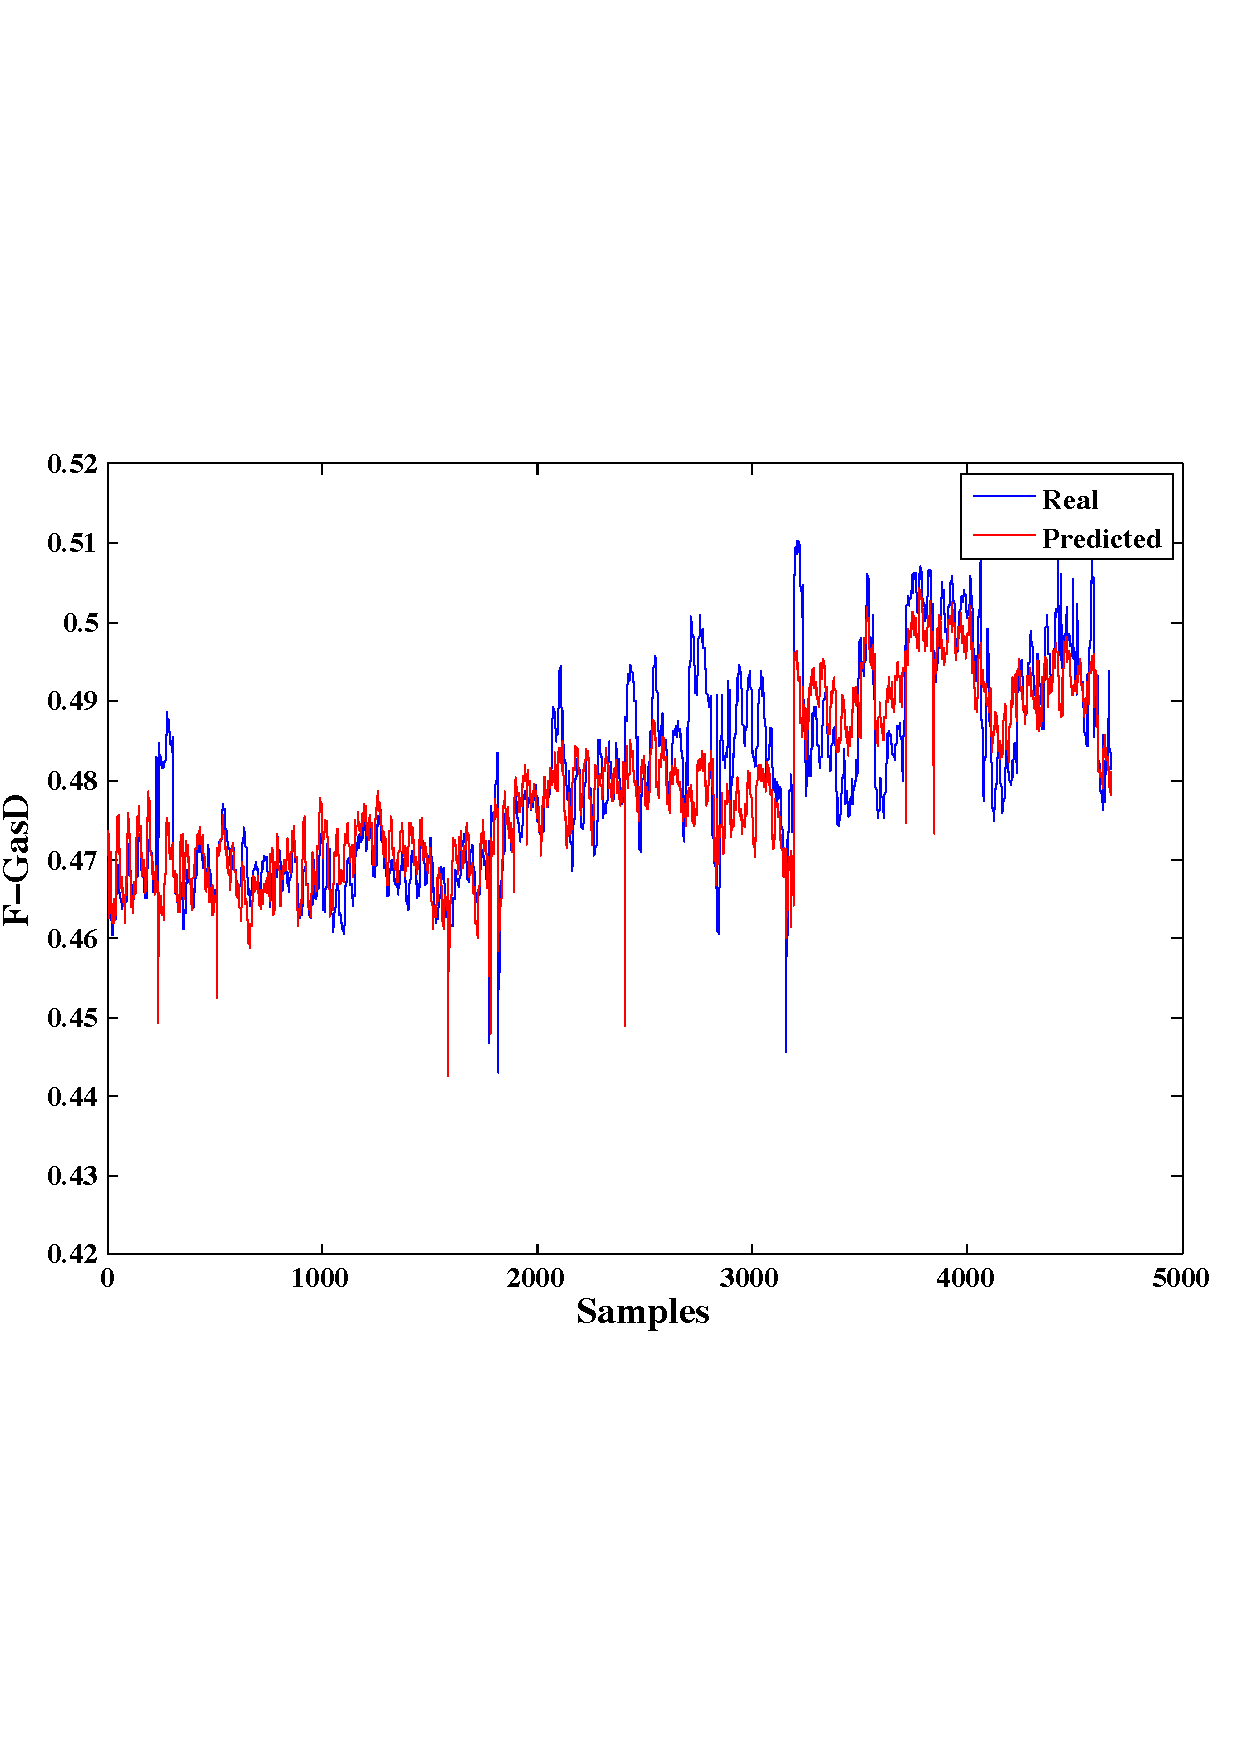
\includegraphics[width=1\textwidth]{ANNengineD.pdf}
\caption{Real data and NN predicted data for the natural gas flow  of Engine A ($F_{GasA}$).}
\label{FengineA}
\end{figure}

\begin{figure}
\centering
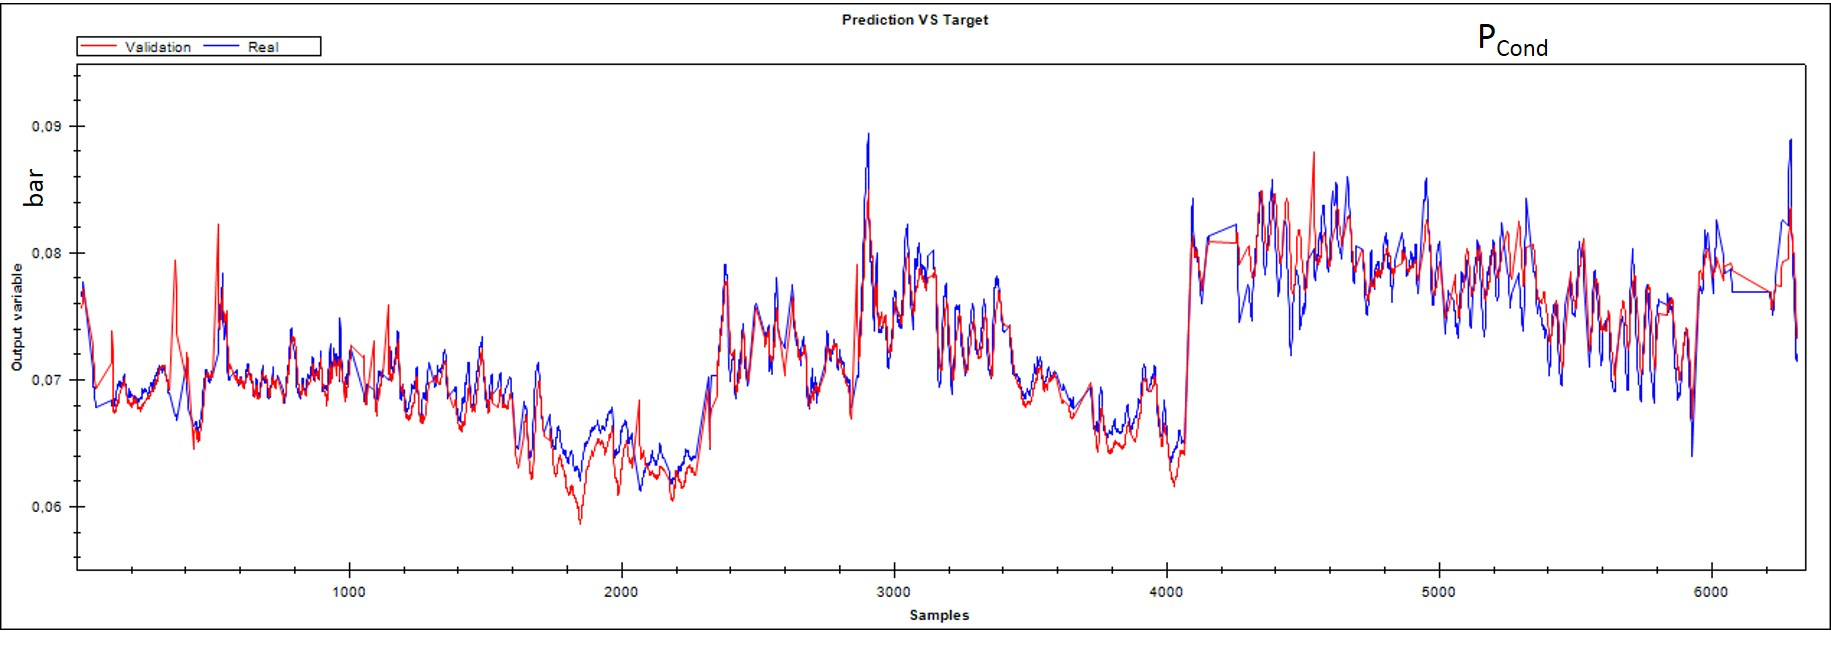
\includegraphics[width=1\textwidth]{ANN-STcond.pdf}
\caption{Real data and NN predicted data for the steam pressure of the condenser  ($P_{Cond}$).}
\label{Pcond}
\end{figure}

\begin{figure}
\centering
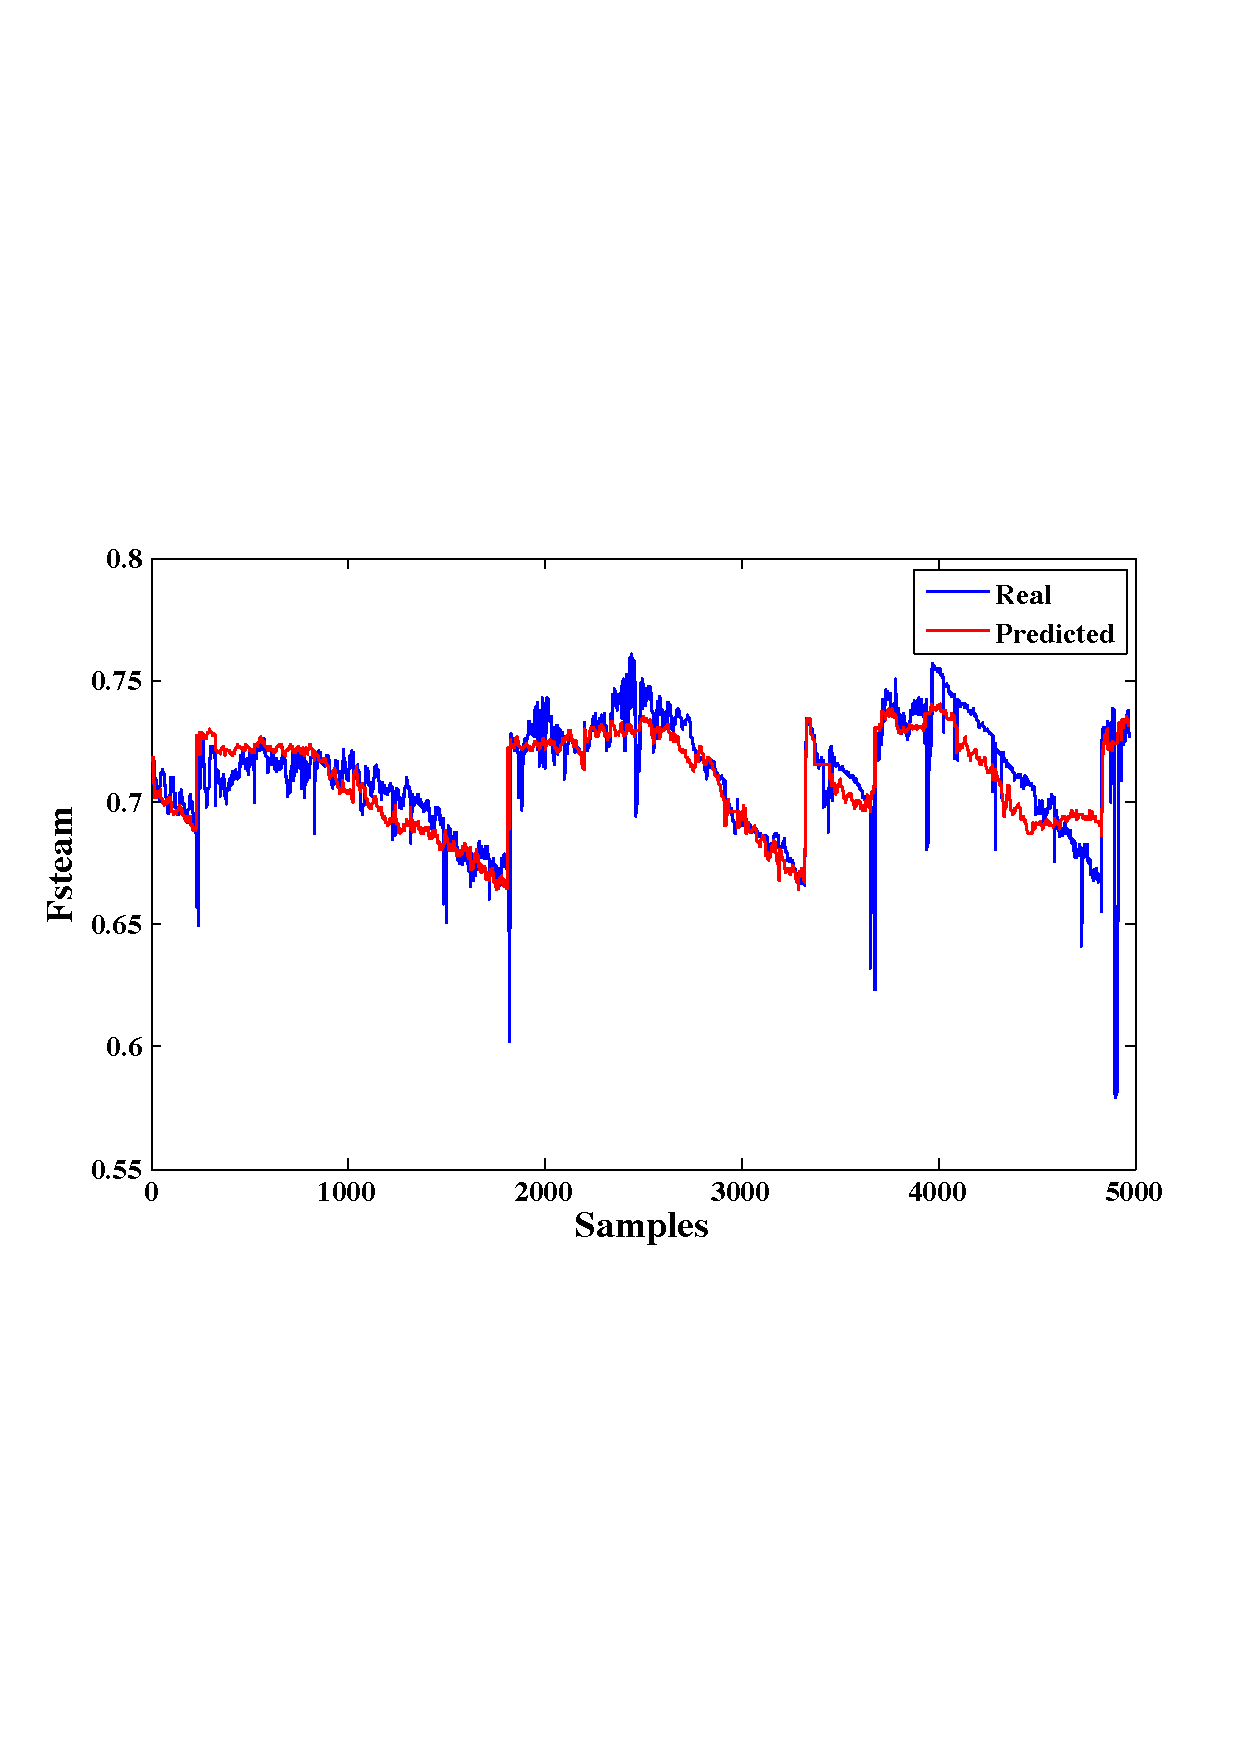
\includegraphics[width=1\textwidth]{ANN-EXHAUSTRECOVERY.pdf}
\caption{Real data and NN predicted data for the steam flow in the boiler($F_{Steam}$).}
\label{Fboiler}
\end{figure}

\begin{figure}
\centering
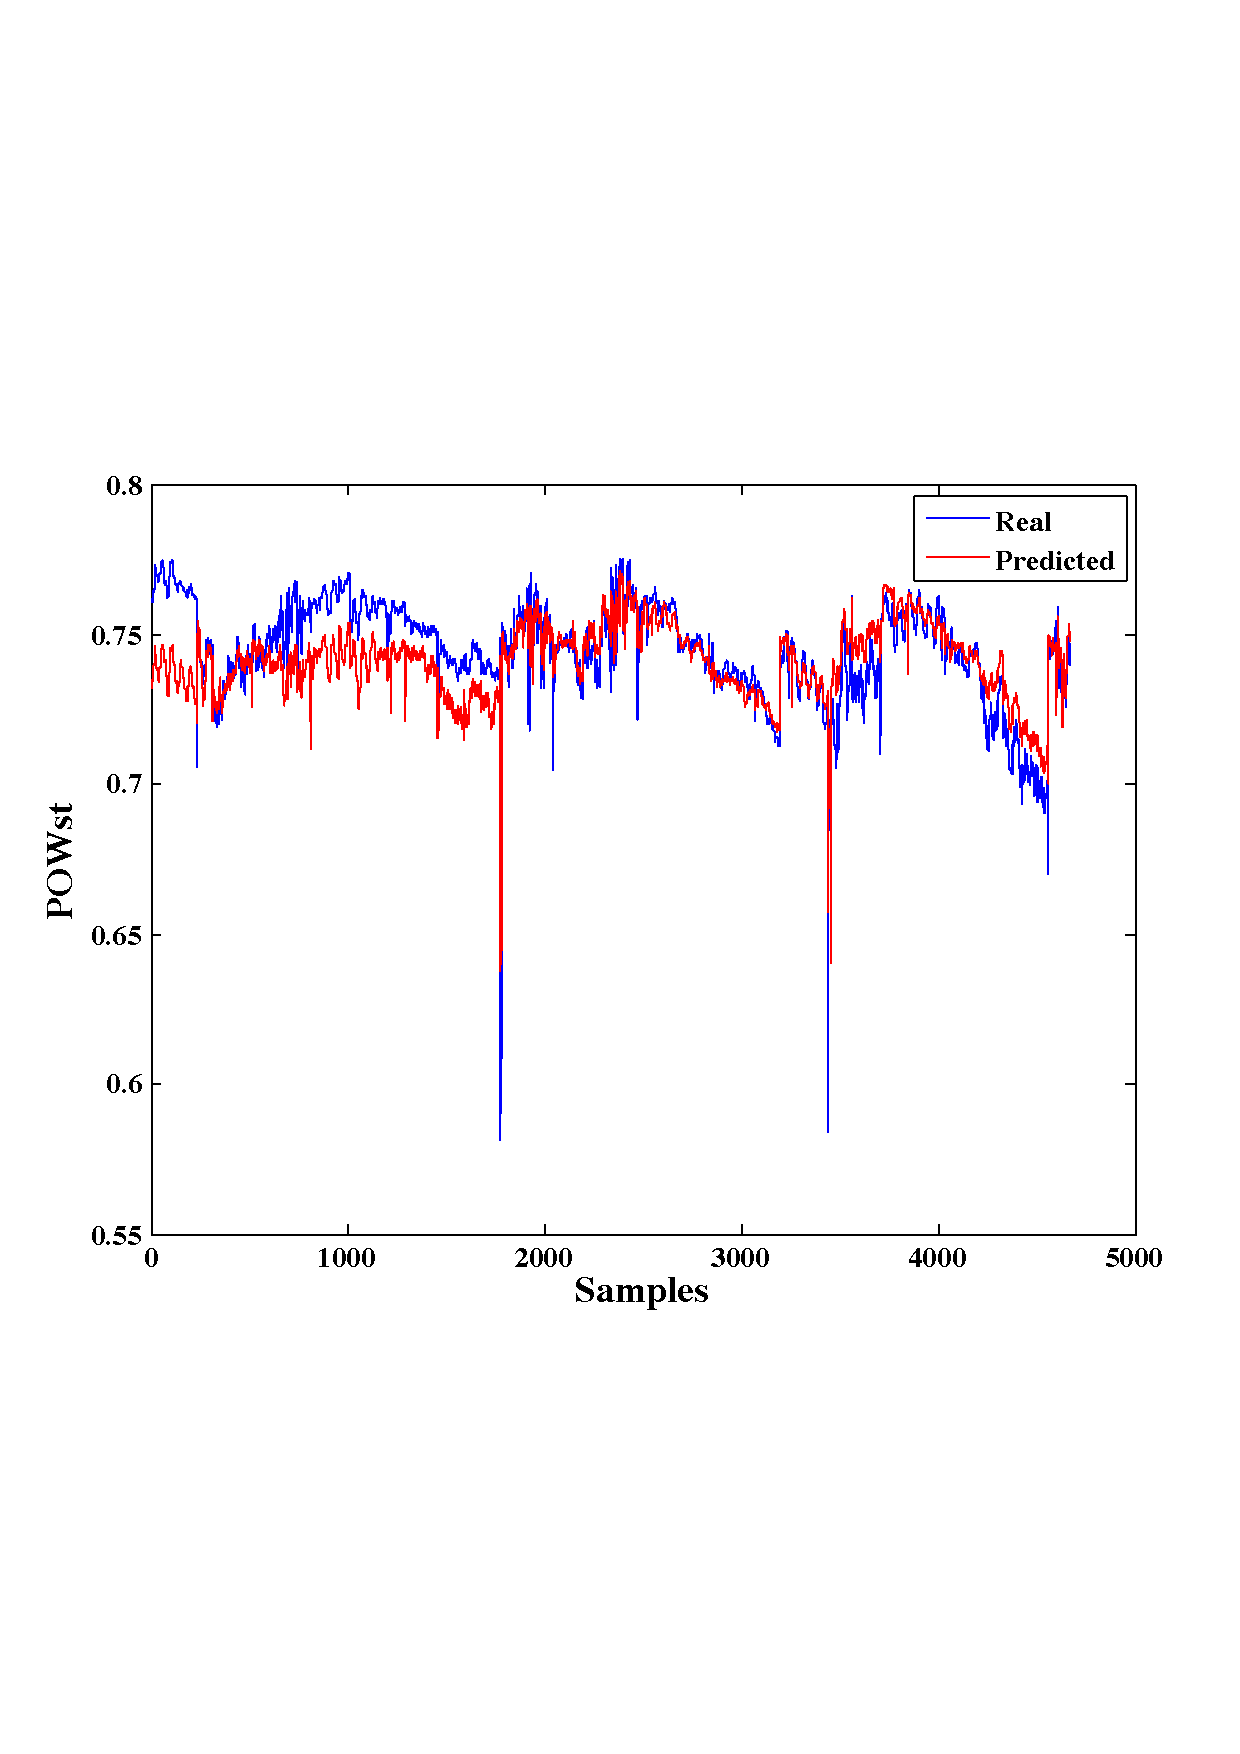
\includegraphics[width=1\textwidth]{ANN-ST.pdf}
\caption{Real data and NN predicted data for the Power generated in the Turbine ($POW_{ST}$).}
\label{Pturbine}
\end{figure}

\begin{figure}
\centering
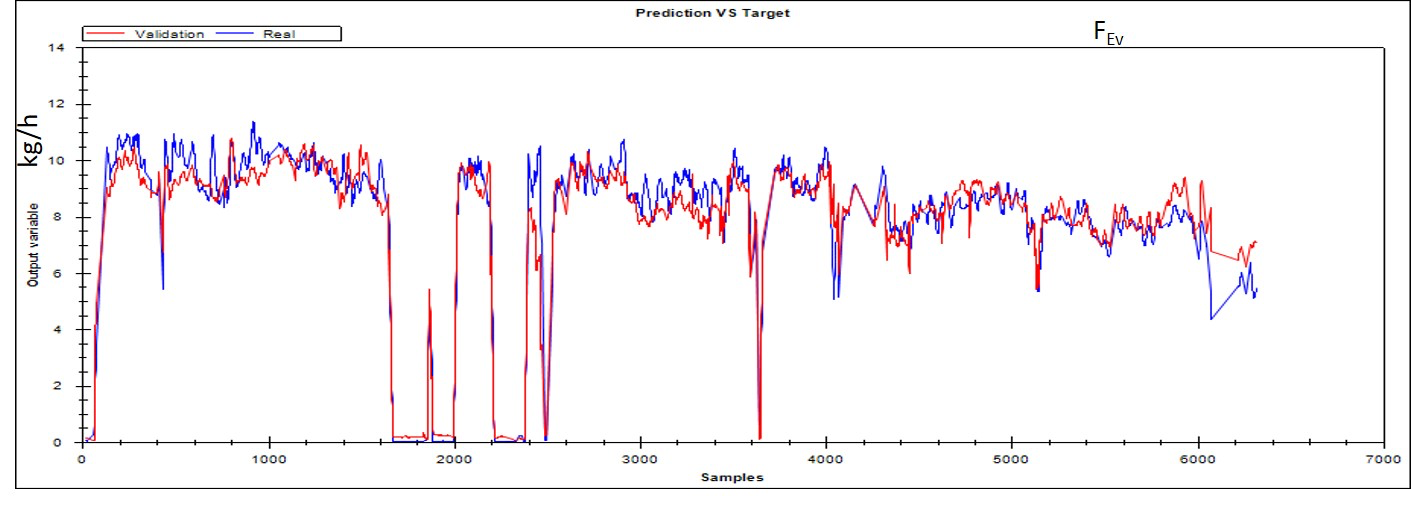
\includegraphics[width=1\textwidth]{ANN-Evaporator.pdf}
\caption{Real data and NN predicted data for the Slurry drying process ($F_{Ev}$).}
\label{PEvaporator}
\end{figure}
